\section{EFT description} \label{sec:EFT_Description}

As di-Higgs in the WW$\gamma\gamma$ final state is predicted in the SM, a search for its SM signature is performed. In order to increase the breadth of the search, the analysis is extended to a search for a variety of EFT scenarios predicting the HH$\rightarrow$WW$\gamma\gamma$ process with varying cross sections. This extension branches from the SM, where the Higgs potential before spontaneous symmetry breaking reads as shown in Equation \ref{eq:SM_H_Potential}, where $\Phi$ is an $SU(2)$ doublet scalar field, and $\phi$ is the real part of its neutral component, equal to $v + H$, where $v$ is the field's vacuum expectation value.

\begin{eqnarray} \label{eq:SM_H_Potential}
  V(\Phi) = - \frac{\mu^2}{2}\left|\Phi \right|^2
  +\frac{\lambda}{4} \left|\Phi \right|^4
\end{eqnarray}

Requiring there be a minimum value of this potential leads to the relations shown in Equation \ref{eq:Minimum_relations}.

\begin{eqnarray} \label{eq:Minimum_relations}
  \lambda = \frac{m_H^2}{2 v^2}, \;\;  \mu^2 = \frac{m_H^2}{2},
  \;\; m_H^2 = \frac{\partial^2 V}{\partial \phi^2}
   \label{eqm-2}
\end{eqnarray}

These relations include a determination of the structure of the Higgs self-coupling, $\lambda$, as a value depending on the Higgs mass $m_{H}$ and Higgs vacuum expectation value (VEV) $v$. After spontaneous symmetry breaking, the leading terms of the Higgs potential look as shown in Equation \ref{eq:HiggsPotential_after_SSB}. 

\begin{eqnarray} \label{eq:HiggsPotential_after_SSB}
  V = \frac{m_H^2}{2}H^2 + \lambda_3 v H^3 + \frac{\lambda_4}{4} H^4,
\quad
 \lambda_3 = \lambda_4 = \lambda_{HHH} = \frac{m_H^2}{2v^2}
\end{eqnarray}

Experimentally measuring $\lambda_{HHH}$ is a crucial test of the SM electroweak symmetry breaking mechanism, in order to compare the experimentally measured value to its SM predictions. Modifications of the Higgs self-coupling coupling ($\lambda_{HHH}$) can only be directly accessed via Higgs pair production, making this analysis a good use-case to search for possible BSM effects on the structure of the Higgs self-coupling. 

In this analysis, the effective Lagrangian \cite{deFlorian:2016spz, Carvalho:2015ttv} used to describe Higgs pair production is shown in Equation \ref{Eq:LagrangianBSM}, with its parameters' mathematical definitions shown in Equation \ref{Eq:LagrangianBSM_params}, and corresponding SM and BSM Feynman diagrams shown in Figure \ref{fig:ggHH_production}.

\begin{equation} \label{Eq:LagrangianBSM}
    \mathcal{L}_{BSM} = -{\textcolor{ForestGreen}{\kappa_{\lambda}}} \lambda^{SM}_{HHH} v H^3 -
      \frac{m_t}{v}({\textcolor{blue}{\kappa_t}} H + \frac{\textcolor{red}{c_2}}{v} H^2)(\bar{t_L}t_R + h.c.)
      + \frac{\alpha_S}{12 \pi v}(\textcolor{red}{c_g} H
      - \frac{\textcolor{red}{c_{2g}}}{2 v}H^2)G^a_{\mu \nu}G^{a, \, \mu \nu}
\end{equation}

\begin{eqnarray}\label{Eq:LagrangianBSM_params}
    &&{\textcolor{ForestGreen}{\kappa_{\lambda}}} = \frac{\lambda_{HHH}}{\lambda_{HHH}^{SM}}, \;
    \lambda_{HHH}^{SM} = \frac{ m^2_{H}}{2v^2}, \;\;
    {\textcolor{blue}{\kappa_{t}}} = \frac{ y_{t}}{y_{t}^{SM}}, \;\;
    y_{t}^{SM} = \frac{\sqrt{2} m^2_{t}}{ v}
\end{eqnarray}

\begin{figure}[!htbp]
  \subfloat[SM-like processes]{%
  \label{SMLO_ggHH_production}
            \begin{minipage}[t]{\linewidth}
                  \begin{center}
                          \raisebox{-0.7\height}{ 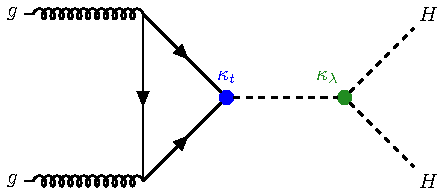
\includegraphics[width=0.45\textwidth]{Sections/HHWWgg/images/EFT_Description/fey_HH_Triangle.pdf} }
                          \raisebox{-0.625\height}{ 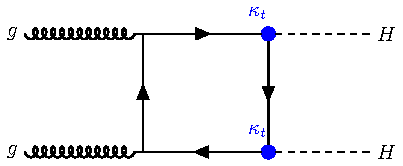
\includegraphics[width=0.45\textwidth]{Sections/HHWWgg/images/EFT_Description/fey_HH_Box.pdf} }
                  \end{center} 
          \end{minipage}%
  }
  
  \subfloat[Pure BSM processes]{%
  \label{BSMLO_ggHH_production}
          \begin{minipage}[t]{\linewidth}
                  \begin{center}
                          \raisebox{-0.7\height}{ 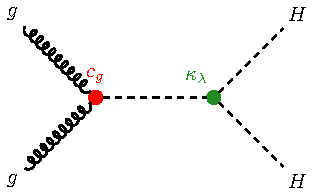
\includegraphics[width=0.30\linewidth,clip]{Sections/HHWWgg/images/EFT_Description/fey_HH_anomal_2_colored.pdf} }
                          \raisebox{-0.7\height}{ 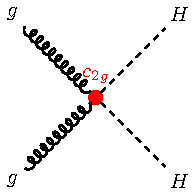
\includegraphics[width=0.20\linewidth,clip]{Sections/HHWWgg/images/EFT_Description/fey_HH_anomal_3_colored.pdf} }
                          \raisebox{-0.7\height}{ 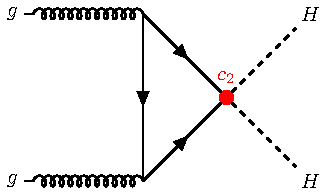
\includegraphics[width=0.30\linewidth,clip]{Sections/HHWWgg/images/EFT_Description/fey_HH_anomal_4_colored.pdf} }
                  \end{center}
          \end{minipage}
  }
  \caption{Feynman diagrams for leading-order Higgs boson pair production via gluon fusion}
  \label{fig:ggHH_production}
  \end{figure}
  

Qualitatively, each of these variables are defined as follows:

\begin{itemize} \label{EFT_parameters_description}
  \item $G^a_{\mu \nu} = \partial_{\mu} G_{\nu}^a - \partial_{\nu} G_{\mu}^a + f^{abc}  G_{\mu}^b G_{\nu}^c$ is the gluon field strength tensor.
  \item $f^{abc}$ is the totally anti-symmetric $SU(3)$ structure tensor.
  \item \textcolor{ForestGreen}{$\kappa_{\lambda}$} is a measure of the deviation of the Higgs boson self-coupling from its SM expectation $\lambda_{HHH}^{SM}$. For example, \textcolor{ForestGreen}{$\kappa_{\lambda}$} = 2 corresponds to a self-coupling with twice the strength as the SM expectation.
  \item \textcolor{blue}{$\kappa_{t}$} is a measure of the deviation of the coupling of a single Higgs boson and two top quarks, called the top Yukawa coupling, from its SM expectation $y_{t}^{SM}$. For example, \textcolor{blue}{$\kappa_{t}$} = 2 corresponds to a top Yukawa coupling with twice the strength as the SM expectation.
  \item \textcolor{red}{$c_{2}$} is the strength of a purely BSM coupling between two Higgs bosons and two top quarks. In the SM this coupling strength equals zero, as the dimension of this added lagrangian term would be non-renormalizable.
  \item \textcolor{red}{$c_{g}$} is the strength of a purely BSM coupling between one Higgs boson and two gluons. In the SM this coupling strength equals zero, corresponding to the fact that gluons are massless in the SM.
  \item \textcolor{red}{$c_{2g}$} is the strength of a purely BSM coupling between two Higgs bosons and two gluons. In the SM this coupling strength equals zero, corresponding to the fact that gluons are massless in the SM.
\end{itemize}

In order to simplify the search of HH models across the entire 5-dimensional phase space and avoid the need to generate simulated events for a large number of points in the 5-dimensional EFT space, a reweighting technique is employed, a set of benchmark EFT points is searched for, and scans of multiple EFT parameters are performed. Within this lagrangian formalization, the differential cross section of of gluon-gluon fusion induced Higgs boson pair production, $\sigma_{HH}$, can be expressed as a polynomial in terms of the EFT model parameters using generator-level information on the HH system as shown in Equation \ref{eq:reweight_eq}.

\begin{equation} \label{eq:reweight_eq}
  \frac{d^2\sigma}{d m_{HH}d|\cos{\theta^*}| } = \sum A_i( m_{HH}, |\cos{\theta^*}| ) \, c_i
\end{equation}

where $c_i$ represents the combinations of couplings defined in \cite{Buchalla:2018yce}, and $A_i( m_{HH}, |\cos{\theta^*}| )$ are known coefficient values. Equation \ref{eq:reweight_eq} is used to extract per event weights, which are normalized by equation \ref{eq:LONLONorm}, where $\sigma_i$ ($\sigma_f$) is the cross section of the initial (final) benchmark point when reweighting i $\rightarrow$ f. This allows one to reweight any HH sample at NLO to any other HH sample at NLO precision. In this analysis, this is used to reweight from a set of generated HH samples at NLO to any point in the 5-dimensional EFT phase space \cite{Carvalho:2016rys,Buchalla:2018yce}. Additionally, when performing DNN trainings in the SL and FH final states, signal samples generated at LO are reweighted to the SM at NLO using this technique in order to provide a larger number of signal events for training.

\begin{equation} \label{eq:LONLONorm}
  w(m_{HH}, |\cos{\theta^*}|) = \frac{d\sigma_f(m_{HH}, |\cos{\theta^*}|)}{d\sigma_i(m_{HH}, |\cos{\theta^*}|)} \cdot \frac{\sigma_i}{\sigma_f}
\end{equation}

With this technique, twenty benchmark scenarios considered in this analysis, chosen as they are largely representative of different kinematic regions of the 5-dimensional EFT phase space \cite{Carvalho:2015ttv,Buchalla:2018yce,Capozi:2019xsi}, are produced via a reweighting of four generated simulation samples at NLO ($\kappa_{\lambda}$ = [0, 1, 2.45, 5]) and are shown in Table \ref{tab:eft_bench}.  

In addition, by considering a linear combination of the four generated simulation samples weighted to their corresponding contribution to arbitrary $\kappa_{\lambda}$ and $c_{2}$ signal hypotheses, scans of these two parameters can be performed in order to constrain their values. The $\kappa_{\lambda}$ parameter also affects the Higgs boson branching ratios and the single Higgs production cross sections because of next-to-leading (NLO) electroweak corrections \cite{Degrassi:2016wml,Maltoni:2017ims}, taken into account when scanning over $\kappa_{\lambda}$ values.

\begin{table}[h]
  \begin{center}
    \begin{tabular}{r|ccccc}
      Benchmark & $\kappa_{\lambda}$ & $\kappa_{t}$ & $c_{2}$	& $c_{g}$ & $c_{2g}$ \\ \hline
      SM &	1.0 & 1.0	 &	0.0		& 0.0	& 0.0 \\ \hline
      1 &	7.5	 & 1.0	 &	-1.0	& 0.0	& 0.0 \\
      2 &	1.0	 & 1.0	 &	0.5		& -0.8	& 0.6 \\
      3 &	1.0	 & 1.0	 &	-1.5	& 0.0	& -0.8 \\
      4 &	-3.5 & 1.5  &	-3.0	& 0.0	& 0.0 \\
      5 &	1.0	 & 1.0	 &	0.0		& 0.8	& -1 \\
      6 &	2.4	 & 1.0	 &	0.0		& 0.2	& -0.2 \\
      7 &	5.0	 & 1.0	 &	0.0		& 0.2	& -0.2 \\
      8 &	15.0 & 1.0	 &	0.0		& -1	& 1 \\
      9 &	1.0	 & 1.0	 &	1.0		& -0.6	& 0.6 \\
      10 &	10.0 & 1.5   &	-1.0	& 0.0	& 0.0 \\
      11 &	2.4	 & 1.0	 &	0.0		& 1		& -1 \\
      12 &	15.0 & 1.0	 &	1.0		& 0.0	& 0.0 \\[0.5ex] \hline 
      8a &  1.0  & 1.0   &  0.5   & $\frac{0.8}{3}$ & 0.0 \\[0.5ex] 
      1b &  3.94 & 0.94  & $\frac{-1}{3}$ & 0.75 & -1 \\[0.5ex] 
      2b &   6.84 & 0.61 &  $\frac{1}{3}$ &  0.0 & 1.0 \\[0.5ex] 
      3b &   2.21 & 1.05 & $\frac{-1}{3}$ &  0.75 &  -1.5 \\[0.5ex] 
      4b &   2.79 & 0.61 &  $\frac{1}{3}$ & -0.75 &  -0.5 \\[0.5ex] 
      5b &   3.95 & 1.17 & $\frac{-1}{3}$ & 0.25 &  1.5 \\[0.5ex] 
      6b &   5.68 & 0.83 &  $\frac{1}{3}$ & -0.75 &  -1.0 \\[0.5ex] 
      7b &   -0.10 & 0.94 &         1.0 & 0.25 & 0.5 \\
    \end{tabular}
  \end{center}
  \caption{Parameter values of the 20 EFT benchmarks and the Standard Model. \label{tab:eft_bench}}
\end{table}
